\documentclass{article}
\usepackage{amsmath, amsfonts, amssymb, amsthm}
\usepackage{enumitem, tikz}

\title{PS06-03}
\date{\today}

\begin{document}
\maketitle
Pictured below is the the $TM-23$ $M$, which can be expressed as $\langle Q, \Sigma, \Gamma, \vdash, \_, \delta, s, t, r\rangle$.\\
Where $\Sigma = \{0,1\}$,\\
$\Gamma = \{\vdash, x, y, \_\} \cup \Sigma$,\\
$s = q0$,\\
$t = h-t$,\\
$r = h-r$.\\
This machine recognizes $A ::= \{0^n1^n:n\geq1\}$, which no DFA can recognize.
\begin{center}
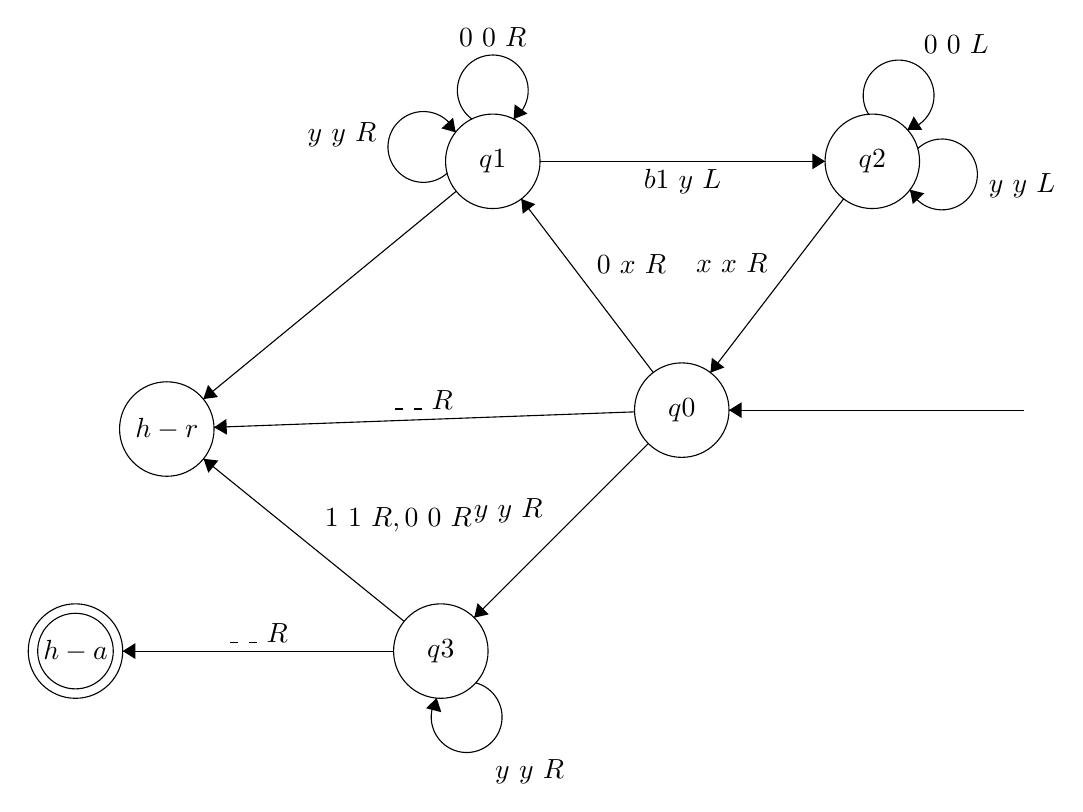
\begin{tikzpicture}[scale=0.2]
\tikzstyle{every node}+=[inner sep=0pt]
\draw [black] (48.9,-26.7) circle (3);
\draw (48.9,-26.7) node {$q0$};
\draw [black] (36.9,-10.9) circle (3);
\draw (36.9,-10.9) node {$q1$};
\draw [black] (61,-10.9) circle (3);
\draw (61,-10.9) node {$q2$};
\draw [black] (33.6,-42) circle (3);
\draw (33.6,-42) node {$q3$};
\draw [black] (16.2,-27.9) circle (3);
\draw (16.2,-27.9) node {$h-r$};
\draw [black] (10.4,-42) circle (3);
\draw (10.4,-42) node {$h-a$};
\draw [black] (10.4,-42) circle (2.4);
%\draw [black] (70.6,-27) circle (5);
\draw [black] (47.09,-24.31) -- (38.71,-13.29);
\fill [black] (38.71,-13.29) -- (38.8,-14.23) -- (39.6,-13.62);
\draw (43.47,-17.4) node [right] {$0\mbox{ }x\mbox{ }R$};
\draw [black] (35.577,-8.22) arc (234:-54:2.25);
\draw (36.9,-3.65) node [above] {$0\mbox{ }0\mbox{ }R$};
\fill [black] (38.22,-8.22) -- (39.1,-7.87) -- (38.29,-7.28);
\draw [black] (39.9,-10.9) -- (58,-10.9);
\fill [black] (58,-10.9) -- (57.2,-10.4) -- (57.2,-11.4);
\draw (48.95,-11.4) node [below] {$b1\mbox{ }y\mbox{ }L$};
\draw [black] (34.008,-11.651) arc (312.2882:24.2882:2.25);
\draw (29.55,-9.2) node [left] {$y\mbox{ }y\mbox{ }R$};
\fill [black] (34.54,-9.06) -- (34.38,-8.13) -- (33.64,-8.81);
\draw [black] (63.878,-10.097) arc (133.32456:-154.67544:2.25);
\draw (68.36,-12.43) node [right] {$y\mbox{ }y\mbox{ }L$};
\fill [black] (63.39,-12.7) -- (63.57,-13.62) -- (64.3,-12.93);
\draw [black] (60.767,-7.921) arc (212.19859:-75.80141:2.25);
\draw (66.33,-4.08) node [above] {$0\mbox{ }0\mbox{ }L$};
\fill [black] (63.22,-8.9) -- (64.17,-8.9) -- (63.63,-8.05);
\draw [black] (59.18,-13.28) -- (50.72,-24.32);
\fill [black] (50.72,-24.32) -- (51.61,-23.99) -- (50.81,-23.38);
\draw (54.38,-17.39) node [left] {$x\mbox{ }x\mbox{ }R$};
\draw [black] (46.78,-28.82) -- (35.72,-39.88);
\fill [black] (35.72,-39.88) -- (36.64,-39.67) -- (35.93,-38.96);
\draw (37.88,-33.87) node [above] {$y\mbox{ }y\mbox{ }R$};
\draw [black] (35.808,-44.014) arc (75.37062:-212.62938:2.25);
\draw (39.24,-48.85) node [below] {$y\mbox{ }y\mbox{ }R$};
\fill [black] (33.34,-44.98) -- (32.66,-45.63) -- (33.63,-45.88);
\draw [black] (45.9,-26.81) -- (19.2,-27.79);
\fill [black] (19.2,-27.79) -- (20.02,-28.26) -- (19.98,-27.26);
\draw (32.47,-26.7) node [above] {$\_\mbox{ }\_\mbox{ }R$};
\draw [black] (34.58,-12.8) -- (18.52,-26);
\fill [black] (18.52,-26) -- (19.45,-25.87) -- (18.82,-25.1);
\draw [black] (31.27,-40.11) -- (18.53,-29.79);
\fill [black] (18.53,-29.79) -- (18.84,-30.68) -- (19.47,-29.9);
\draw (30.91,-34.46) node [above] {$1\mbox{ }1\mbox{ }R,0\mbox{ }0\mbox{ }R$};
\draw [black] (30.6,-42) -- (13.4,-42);
\fill [black] (13.4,-42) -- (14.2,-42.5) -- (14.2,-41.5);
\draw (22,-41.5) node [above] {$\_\mbox{ }\_\mbox{ }R$};
\draw [black] (70.6,-26.7) -- (51.9,-26.7);
\fill [black] (51.9,-26.7) -- (52.7,-27.2) -- (52.7,-26.2);
\end{tikzpicture}
\end{center}

%An example of a DFA that can recognize a language that a $TM-23$ cannot is a DFA that recognizes $B ::= \{0^n: n \text{is an arbitrarily large prime}\}$. Even though a Turing machine can count occurances or binary with relatively few states, matching that number if it was very large would be impossible. For instance, lets say that $n$ is a 23 digit prime. A DFA would have $n$ states, the last of which being an accept state. With very few states, a Turing machine can tally 0s and write them in decimal. ($1,2,3,4,5,6,7,8,9,0 \in \Gamma$), but for each decimal digit, the Turing machine will need a state to match it and prove equality. If $n$ is 23 digits, 
An example of a regular language that cannot be recognized by a $TM-23$ machine is $B ::= \{0^n:n \mod 29 = 7 \text{ or } 13\}$ A DFA would have 29 states, 2 of which would be accept states(the 7th and the 13th). The efficient way a turing machine calculates mods is by removing the divisor's amount of 0s until there is fewer than that number, at which point, the remaining number of 0s is the answer. The machine could use the same strategy as the DFA to count 0s, but that would result in too many states. Another way would be to use a counter, like the one in the online Turing simulator used last problem set(for the binary to decimal converter), which would remove zeros and check to see if the decimal counter of zeros was 7, 13 or 29. If it was 7 or 13, it would halt-accept, and if it was 29, it would reset the number to 0. The tape alphabet would be 0-9, $\vdash$ and $\textvisiblespace$. The Tape alphabet length does not violate the $TM-23$ rule, but the complexity of the system is too much to be expressed in 23 states.
\end{document}
